\newcommand{\CLASSINPUToutersidemargin}{1.5in}
\documentclass[10pt,final,journal]{IEEEtran}
\usepackage{graphicx}
\usepackage{algorithmic}

\begin{document}
\title{Troups: Scalable Transactions for BigTable datastores}
\author{Benjamin Busjaeger, Jonathan Chu, Daniel Ormond \\
\{busjaeg2, jmchu2, ormond1\}@illinois.edu}
\date{Feb 2012}
\maketitle

\begin{abstract}
Troups is a novel transaction manager for cloud datastores of the BigTable family that provides full ACID transactions across co-located data items. It includes a mechanism for grouping related rows and an algorithm that aids users in deciding what groups to form by identifying data types and items frequently accessed together in transaction logs. This allows us to improve the consistency guarantees of these systems without significantly impacting their high scalability or availability.
\end{abstract}

\begin{IEEEkeywords}
cloud, data storage, BigTable, transaction processing
\end{IEEEkeywords}

\section{Introduction}
Cloud platforms like Google and Amazon store vast amounts of data. This is in part because they pool resources to efficiently serve multiple tenants and in part because the volume of data produced by applications and users has significantly increased in recent years. At the same time users expect their data to always be quickly accessible anywhere and they have little tolerance for data loss or inconsistencies. Studies like ~\cite{Ramsay:1998} have shown that users quickly become  irritated by long response times and take their business elsewhere. Unfortunately, per Brewer's conjecture ~\cite{gilbert2002brewer}, it is not possible to maximize all of these goals simultaneously. These challenges have forced a change in the way data is stored and processed in the cloud.

Traditional relational database management systems (RDBMSs) are designed to provide high consistency by giving users the impression of a single system image. The conventional approach of improving availability and performance of these systems by purchasing more powerful and resilient hardware has obvious scalability limitations and is often not cost effective. The alternative of clustering traditional RDBMSs across less expensive hardware has its own set of challenges, since the single system objective implies high overhead from frequent distributed transactions and limited partition tolerance. Popular open source databases like MySQL have been shown to only scale to a small number of nodes ~\cite{Malkowski:2010:EAD:1774088.1774449} and commercial RDBMSs have similar limitations ~\cite{Campbell:2010:ESF:1807167.1807280}.

In response to the lack of scalability and high operational cost of traditional RDBMSs, large Internet companies have recently developed their own data storage solutions. Some notable examples of these so called NoSQL datastores are Google's BigTable ~\cite{Chang:2006:BDS:1267308.1267323}, Yahoo's PNUTS ~\cite{Cooper:2008:PYH:1454159.1454167}, and Amazon's Dynamo ~\cite{DeCandia:2007:DAH:1323293.1294281}. These architectures are radical departures from traditional RDBMSs in that they do not expose complex query operations and provide only limited consistency guarantees. This allows them to more efficiently partition data across dynamically scalable clusters and to isolate faults to subsets of the system.

Many cloud applications, like search index construction, can easily tolerate relaxed consistency guarantees. However, other applications, like emerging OLTP multi-tenant platforms, have strong isolation and atomicity requirements. Without sufficient transaction support built into the infrastructure, the burden of ensuring data integrity is ultimately placed on application developers.

Troups, which stands for Transaction Groups, aims to improve the transactional capabilities of NoSQL datastores in the BigTable family without compromising their scalability. To this end, it extends the BigTable programming model with the ability to group related rows in order to co-locate their data for efficient transaction processing. Troups also supports cross-group transactions, but tries to minimize their use to avoid two-phase commit overhead. Our transaction manager is novel in that it is designed as an observer, which means it extends BigTable without requiring changes and it is theoretically portable across datastores that satisfy the constraint model. We have also developed a set of group detection and placement algorithms to facilitate and optimize the task of identifying groups and allocating them to servers. In summary, our main contributions to the research field are:

\begin{enumerate}
\item A novel transaction manager for BigTable-like datastores that enables full ACID transactions at large scale for applications that exhibit transaction locality.
\item A set of group detection and Time Swap placement algorithms based on transaction logs.
\end{enumerate}

\section{Related Work}
Research on cloud-scale OLTP systems generally falls into two categories. On one hand, numerous approaches have been proposed recently for extending cloud datastores with more powerful transaction models. On the other hand, several recent publications describe how to adapt RDBMSs to make them more suitable for cloud workloads. The common theme across these approaches is a departure from full featured ACID transactions across the full data set. The proposals either reduce transaction isolation levels to make global transactions feasible or restrict serializable transactions to a subset of the data. In the latter case selection of these subsets is critical for ensuring efficient transaction processing, so algorithms have emerged to automate this process. We will first examine and classify OLTP cloud datastore architectures and subsequently survey relevant work on optimized data partitioning.

\subsection{OLTP Cloud Datastores}
\emph{Cloud SQL Server} ~\cite{Campbell:2010:ESF:1807167.1807280, Bernstein:2011:AMS:2004686.2005651}, \emph{ElasTraS} ~\cite{Das:2009:EET:1855533.1855540, Das:2010:EAE}, and \emph{Relational Cloud} ~\cite{Curino:2011:JPMWMBZ11} describe approaches for horizontally scaling out different relational DBMSs. Cloud SQL Server augments Microsoft SQL Server with partitioning and primary-copy replication. Serializable ACID transactions are supported, but limited to a single partition, which can be a whole logical database, referred to as a table group, or a set of rows from a table group that have been assigned a common partitioning key by the user. ElasTraS uses hierarchical schema-level partitioning and also restricts transactions to one partition. It differs from Cloud SQL Server in that it decouples storage from metadata management through the use of a distributed file system. This allows for a dynamic mapping between partitions and nodes. Relational Cloud combines a workload-aware approach for efficient data placement with a graph-based partitioning algorithm for data co-location discussed in the next section. ACID transactions are supported within and across partitions. Although our approach is not targeted at RDBMSs, it uses similar partitioning techniques.

\emph{Percolator} ~\cite{Peng:2010:LIP:1924943.1924961}, \emph{HBaseSI} ~\cite{Zhang:2010:5697970} and \emph{ReTSO} ~\cite{Junqueira:2011:LTS:2056318.2057148} are different approaches for adding global transactions with snapshot isolation \footnote{See Background section for details on snapshot isolation} semantics to BigTable-like datastores. Percolator is specifically designed to allow incremental search index construction, so it is optimized for throughput and not suitable for latency-sensitive applications. HBaseSI is a pure client API that uses a set of custom tables and atomic test-and-set operations to manage transactions without central coordination. ReTSO implements a lock-free commit algorithm using a centralized Transaction Status Oracle. The benefit of these approaches is that they do not rely on data co-location to support one-phase commit transactions. The downside is weaker isolation. Troups does not rely on a centralized concurrency control component, so it can offer stronger isolation, but it is less suitable for transactions that span any data in the cluster. Our approach adopts several ideas presented in ReTSO to implement efficient and non-invasive concurrency control.

\emph{G-Store} ~\cite{Das:2010:GSD:1807128.1807157} and \emph{CloudTPS} ~\cite{Wei:2011:5740834} build transaction capabilities targeted at specific use cases on top of BigTable-like datastores. G-Store introduces a key group protocol to provide ACID transactions over dynamically selected key sets. It is intended for applications which need to execute transaction across frequently changing groups of entities, that are non-overlapping, so it has limited applicability. CloudTPS is designed for web application workloads and assumes short-lived transactions that access small data sets known prior to starting the transaction. It interposes a group of Local Transaction Managers (LTMs) between clients and datastores which load data items and transaction state into memory for efficient processing. This implies the need for a separate server cluster with its own fail-over and recovery mechanisms.

\emph{MegaStore} ~\cite{Furman:2008:8530095, Baker:2011:8530095} tries to bridge the gap between RDBMSs and NoSQL datastores by augmenting BigTable with a declarative schema language. It provides strong consistency guarantees within fine-grained partitions, called entity groups, and ensures high availability by synchronously replicating mutations across datacenters. Troups is closely related to Megastore's transaction manager, but differs in several ways. In Megastore groups are the units of concurrency control and logging to enable wide-area network replication. Mutations are first appended to the replicated log and then applied to the datastore after commit. Reads within groups block until changes are applied, whereas reads across groups may not see the latest committed data. In Troups the unit of concurrency control is a cell and the log is tablet-scoped. This enables a high degree of concurrency and batch commit optimizations across groups. Mutations are directly written into the datastore and filtered for read operations. Therefore, readers can see the last written mutation, even if it has not been committed yet. The approaches also differ in how groups are defined, in Megastore entity groups are statically declared in the schema, whereas in Troups groups are dynamically formed based on programmatic group policy functions.

\emph{Deuteronomy} ~\cite{Levandoski:2011:8530161} is noteworthy, because it aims to decouple transaction management from the underlying datastore, a goal shared by our work. To this end, it defines a transaction component (TC) capable of providing full ACID transactions for any datastore that implements a well-defined data component (DC) interface. The TC applies concurrency control and undo/redo logging at the logical record level as opposed to at the physical page level. Our transaction manager also operates against an abstract datastore contract. Our approach differs from Deuteronomy in that it uses different concurrency control and recovery algorithms and does not rely on a centralized transaction manager.

Table ~\ref{classification} summarizes the classification discussed above.

\begin{table}[!t]
\renewcommand{\arraystretch}{1.3}
\caption{OLTP Cloud Data Store Classification}
\label{classification}
\centering
\begin{tabular}{|c|c|c|c|}
\hline
\bfseries Data Store  & \bfseries Data Model & \bfseries  Part. & \bfseries Isolation \\
\hline
\hline
Cloud SQL & relational & yes & serializable \\
ElasTraS & relational & yes & serializable \\
Rel. Cloud & relational & yes & serializable \\
Percolator & BigTable & no & snapshot \\
HBaseSI & BigTable & no & snapshot \\
ReTSO & BigTable & no & snapshot \\
G-Store & BigTable & yes & serializable \\
CloudTPS & BigTable & no & serializable \\
Megastore & BigTable & yes & serializable \\
Deuteronomy & agnostic & no &serializable \\

\hline
\end{tabular}
\end{table}

\subsection{Paritioning Algorithms}
There are multiple partitioning algorithms in use and in study currently.  Not all of the algorithms have the same goal.  Hash-based algorithms help scale the database by evenly distributing the data on different nodes while other algorithms have a more specific goal to reduce transaction overhead.

Schism ~\cite{Curino:2010:SWA:1920841.1920853} is a static partitioning algorithm to reduce distributed transactions for SQL datastores. It uses transaction logs to determine how to partition data. The transaction anaylsis is similar to the work done by Chun-Hung et al.~\cite{chun:2002} It significantly improves performance compared to hash-based and even manual partitioning techniques. These static algorithms are a good starting point for our work and would likely yield better results for key/value stores given their simplified data access model. Also, an incremental version of these algorithms may scale better than the static equivalent, since it may be able to consider only new transaction log entries in each iteration. Another option would be to use a probabilistic algorithm.

Hehme and Bruno ~\cite{Nehme:2011:APD:1989323.1989444} present and algorithm that deeply integrates directly with the parallel query optimizer in Microsoft SQL Server.  Their algorithm provides a static data partitioning recommendation.  Their goals was to provide a data partition strategy in less time than other less deeply integrated solutions.


\section{Background}

\subsection{BigTable}
BigTable ~\cite{Chang:2006:BDS:1267308.1267323} is a distributed storage system developed by Google to efficiently store large amounts of data (petabytes) across many machines (1000s). Data is stored in tables, which are multidimensional maps that index values by a triple consisting of row key, column key, and timestamp. Tables are sparse, meaning only cells that contain data are persisted, and they are sorted in lexicographical order by row key. Each table is dynamically partitioned into ranges of rows, called \emph{tablets}, which are assigned to \emph{tablet servers} by a dedicated \emph{master}. Tablets are reassigned in case of server failure or overload and they are automatically split or merged with other tablets if their size exceeds or falls below certain thresholds. \emph{Clients } access data by first looking up the locations of tablet servers that currently serve the tablets containing relevant rows and then issuing operations against these tablet servers. If the row locations change in between these two steps, the client retries.

Supported operations include read, write, and delete for single rows, batch operations across rows, and scanners with filters to iterate over a subset of rows. The server-side scripting language Sawzall ~\cite{Pike:2005} can be used for more complex read-only queries. Single-row operations are atomic and transactions across multiple operations that access the same row are also supported. Note that single-row transactions can be implemented efficiently in this model, since data in a single row is always stored on the same tablet server. Transactions for operations that span multiple rows are not supported.

Tablets are physically stored in the Google File System (GFS) ~\cite{Ghemawat:2003:GFS:1165389.945450} as large immutable SSTable files. To make small mutations efficient, BigTable first writes them into a redo log and then stores them in an in-memory data structure called \emph{memtable}. The memtable is periodically written to new SSTables and SSTables are iteratively merged through a \emph{compaction} process. The redo log is scoped to tablet servers to reduce disk seeks, so if a tablet server crashes, the log has to be split across tablet servers that are assigned to recover the tablets. Recovery consists of replaying any mutations that have not been stored in SSTables into the new memstore. To avoid this overhead when moving tablets between servers, the source server compacts the tablet once before and once after closing.

BigTable was recently enhanced with Coprocessors which allow executing code directly on tablet servers similar to stored procedures in traditional database systems ~\cite{Dean:2009}. Coprocessors are attached to tablets and share their lifecycle. Clients can invoke coprocessors through a high-level call interface that resolves the location of Coprocessors based on rows. HBase, the main open source implementation of BigTable, also offers Coprocessor \emph{Observers}, which receive notifications about various kinds of tablet lifecycle and data access operations. They are similar to triggers in traditional database systems.

\subsection{Multiversion Concurrency Control}
Multiversion concurrency control (MVCC) ~\cite{Bernstein:1983:MCC:319996.319998} synchronizes concurrent access to data items by having each write operation produce a new version of the data and by mapping each read operation to one of these versions. MVCC allows for a higher degree of concurrency than monoversion protocols, because reads can be served from older versions while newer ones are being created. It also facilitates recovery, since undoing a write means to simply delete the created version. These benefits come at the cost of additional storage needed to keep multiple versions around. Many MVCC protocols with varying degrees of isolation and different conflict resolution behavior have been proposed. We will briefly discuss two relevant optimistic (non-locking) protocols.

\subsubsection{Snapshot Isolation}
In the snapshot isolation protocol ~\cite{Berenson:1995:CAS:568271.223785} each transaction is assigned a unique start timestamp that is larger than any previously assigned timestamp. Each read operation is mapped to the latest version of the data item committed before the transaction started. When a transaction commits, it receives a commit timestamp and writes a new version for each updated data item carrying this timestamps, unless a write conflict is detected, in which case it is aborted. A transaction $t_i$ is in conflict with another transaction $t_j$, if $t_j$ wrote a data item that $t_i$ also wrote and $t_j$'s commit timestamp is in the interval of $t_i$'s start and commit timestamp. This protocol allows for efficient implementation and prevents lost updates, but it does not produce serializable schedules. In particular, it does not prevent the write-skew anomaly depicted in Figure ~\ref{si}, in which two transactions $t_1$ and $t_2$ first read data items $x$ and $y$ respectively and then both update the other data item.

\begin{figure}[!t]
\centering
\hspace*{-.2in}
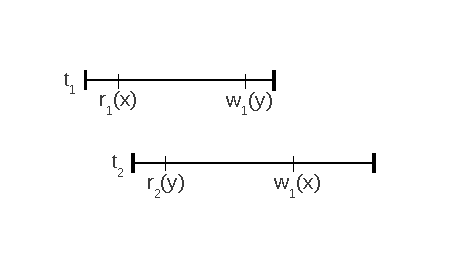
\includegraphics{images/si.pdf}
\caption{Write skew anomaly}
\label{si}
\end{figure}

\subsubsection{Multiversion Timestamp Ordering}
Multiversion timestamp ordering (MVTO) assigns each transaction a unique timestamp that is larger than that of any transaction started before it. It then maps read and write operations onto versions such that the result is equivalent to that of a serial monoversion schedule in which transactions are executed in the order of their timestamps. Operations are scheduled optimistically, so if an ordering conflict occurs that cannot be resolved, one of the transactions is forced to abort and restart.

The concrete protocol consists of the following three rules ~\cite{Weikum:2001:TIS}:
\begin{enumerate}
\item A read operation of some object $x$ by transaction $t_i$ is mapped to the latest version of $x$ written by a transaction that started before $t_i$.
\item A write operation of some object $x$ is rejected and $t_i$ aborted if a transaction that started after $t_i$ has already read a version of $x$ written by a transaction that started before $t_i$. Otherwise, it is transformed into a write operation of version $i$ on object $x$.
\item A commit operation by transaction \emph{i} is delayed until all transactions that have written versions of objects read by \emph{i} have been committed.
\end{enumerate}

MVTO prevents the write-skew anomaly through the second rule: $t_1$ is forced to abort when it attempts to write a new version of $y$, since $t_2$, which started after $t_1$ has alread read the previous version. MVTO is well suited if there is little write contention and has the nice property of being deadlock free, since no locks are used and transactions only ever wait on transactions started before them to commit.

\section{Programming Model}

\subsection{Row Groups}
To enable local transactions across multiple rows, it is necessary to co-locate them in the same tablet and ensure they are not separated as the tablet that contains them is split. Since BigTable sorts tables by row key, using a common row key prefix results in rows being placed next to each other. Such a row key prefix could be a synthetic partitioning key as used in Cloud SQL Server ~\cite{Bernstein:2011:AMS:2004686.2005651} or the key of one of the rows in the group as described in Megastore ~\cite{Baker:2011:8530095}. The latter is an obvious choice if the entities stored in the rows have an inherently hierarchical relationship. We refer to rows with the same prefix as a \emph{row group} and call the prefix the \emph{group key}.

In order for the system to ensure that rows in the same row group are not split, it needs to be made aware of the group key. We do not impose restrictions on how group keys are chosen or how they are prepended as long as the resulting row key complies with the BigTable programming model. Instead, we allow users to define the mapping between row and group keys by implementing a \emph{row group policy} and associating it with the table. The system can use this function to obtain a split point that is guaranteed to be outside of row groups. Note that this scheme preserves query granularity, since it allows for partial key scans as described in ~\cite{George:2011}.

Baker et al ~\cite{Baker:2011:8530095} also describe a pattern for merging multiple tables into a single table by prefixing column keys with table names. Combined with row grouping, this pattern makes it possible to co-locate rows from different tables. Note that such sparse tables are feasible in BigTable, since only cells that contain values are persisted.

\subsection{Group Transactions}
The client API includes methods for demarcating transaction boundaries using the familiar begin-commit-rollback idiom. When starting a new transaction, the client can either create a group or a cross group transaction. In the former case, the transaction will abort and rollback if an operation tries to access rows outside of the group accessed by previous operations in the same transaction. In the latter case, two-phase commit is used to coordinate commits across accessed groups. This implies additional overhead and increases the risk of conflicts, so clients should use cross group transactions sparingly.

Each operation must be enlisted with the transaction before it is executed. Since Troups uses optimistic concurrency control, a transaction may abort while executing an operation or being committed if conflicts are detected that cannot be resolved. In this case, the system rolls back any changes applied by the transaction, so the client can simply retry the transaction.

Troups uses the timestamp dimension to store versions created by different transactions, so timestamps are not available in the client API. This is merely the result of an implementation choice; the system could store multiple versions under a single timestamp as described in ~\cite{Peng:2010:LIP:1924943.1924961} to preserve the timestamp dimension.

\subsection{Group Detection}


\section{Implementation}

\subsection{Timestamp Service}
The MVCC protocols used by our transaction manager require globally unique timestamps to produce serializable schedules across distributed nodes. Since storage capacity is not unlimited in practice, it also needs to know when timestamps are no longer in the range of actively used timestamps so it can free up resources and clean up old versions. We encapsulate this functionality in a \emph{timestamp service (TSS)}. The basic basic function is illustrated in figure ~\ref{ts}.

\begin{figure}[!t]
\centering
\hspace*{-.2in}
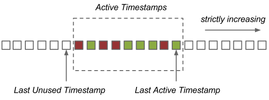
\includegraphics{images/ts-resized.png}
\caption{Timestamp service - green: active timestamps, red: released timestamps}
\label{ts}
\end{figure}

\subsubsection{Protocol}
Clients can \emph{acquire} a timestamp, which is guaranteed to be strictly greater than any currently active timestamp, but not necessarily in sequence. A client that acquires a timestamp becomes its \emph{owner}. An owner can \emph{release} a timestamp explicitly by calling the timestamp service or implicitly by failing, in which case the timestamp service automatically releases it after a certain times has expired. Clients can also inquire if a particluar timestamp has been released and if they are the owner of a particluar timestamp. Alternatively, they can register to be notified when a particular timestamp has been released as a \emph{timestamp listener}. Timestamps between the last unused and first held timestamp are subject to \emph{reclamation}. In the example shown in figure ~\ref{ts} only the leftmost red timestamp is subject to reclamation. Clients can query the value of the currently last reclaimed timestamp or they can register to be notified whenever this value changes as \emph{reclamation listeners}.

While this basic protocol is sufficient if each timestamp has a single owner, it does not address the need for shared ownership, which arises when multiple clients need to hold a timestamp. To support this case, we extended the basic protocol with a \emph{participant} role. After an owner has acquired a timestamp, participants can acquire \emph{references} to it, which are uniquely identified for a particular timestamp. If the owner explicitly or implicitly releases the timestamp at this point, it is marked as released, so the semantics are the same as in the basic protocol. However, the owner can decide to \emph{persist} a set of references. After such a call, the timestamp can only be reclaimed once all participants have explicitly released their references, even if the owner releases the timestamp. In the shared protocol clients can inquire if a reference is held (by them) and if it is persisted. Clients can also register to be notified when a reference is released as a \emph{participant listener}.

\subsubsection{Implementation}
The timestamp service is implemented on top of Zookeeper ~\cite{Hunt:2010:ZWC:1855840.1855851}. Zookeeper is highly available coordination service based on the Paxos algorithm ~\cite{Lamport:1998:PP:279227.279229, Lamport:2001:PMS}, which exposes primitives that map well to the timestamp protocol functions. Basic timestamps are represented as sequential ephemeral nodes. Shared timestamps are represented as sequential persistent nodes with a special ephemeral child node representing the owner role. References are mapped to sequential ephemeral child nodes under the timestamp. To persist a set of references, their identifiers are written into the timestamp node. When a reference is explicitly released, it's ID is removed from the timestamp node. Once all IDs have been removed, the timestamp is considered released. Watches are used to implement the various notification types.

Timestamp reclamation is performed asynchronously by a dedicated reclaimer thread running on one of the tablet servers. The reclaimer periodically scans timestamps to find the first held timestamp in an attempt to move up the last unused timestamp pointer, which is stored in a separate Zookeeper node. In the process it also deletes any shared nodes that have been released, but not properly removed. The scan can be efficiently implemented, because it takes only a single call to retrieve the names of all timestamp nodes from Zookeeper. The client then sorts the timestamps, since Zookeeper makes no ordering guarantees and iterates through them to inquire whether they have been released. If shared timestamps are used sparsely, it typically takes only one Zookeeper call to verify that the first timestamp in the list is still active. To decide which tablet server should run the timestamp reclaimer at any given time, we use a leader election algorithm implemented on top of Zookeeper.

\subsection{Transaction Management}
Transactions are implemented by two components: a \emph{transaction client (TC)} which augments the BigTable client and a \emph{transaction manager (TM)} which augments BigTable's tablet servers. The transaction manager is a special Coprocessor that exposes transaction lifecycle operations through a Coprocessor Endpoint interface and intercepts data access operations through the Coprocessor Observer interface. As such, one instance of the transaction manager is associated with each tablet in the system and its lifecycle is tied to the tablet lifecycle.


Figure TODO illustrates how group transactions are processed. Once the first operation is enlisted with the transaction, the TC computes the group key using the row group policy specified for the table. If no row group policy is specified, each row is treated as a separate group. It then invokes the TM for the row through the Coprocessor Endpoint interface to start a new transaction for the group. The TM acquires a new timestamp as the transaction identifier (TID) from the TSS, establishes the transaction state, and returns the TID to the TC. The TC annotates the operation with the returned TID before returning. On subsequent enlist calls, the TC merely checks that the row accessed by the operation is in the same row group as the row of the initial operation.

When the data access operations are submitted to the tablet server, the TM intercepts them before and after they are executed. It extracts the annotated TID to lookup the transaction state, logs the operations to enable recovery, and enforces the concurrency control protocol. This may include aborting transactions in case irresolvable conflicts are detected. When the TC receives a commit or abort, it forwards it to the TM to complete the transaction.

Cross group transactions are handled slightly differently. The TC first acquires a shared timestamp from the TSS to use as the global TID. Whenever it receives a request to enlist a new operation, it computes the row group for it and if it has not seen it, asks the corresponding TM to join the transaction for the given group. When the TM receives a join request, it acquires a reference to the timestamp, sets a listener on the timestamp, and returns its participant ID. The TC then registers as a participant listener on the ID and returns the annotated operation. The listeners allow both the TC and TM to quickly abort the transaction in case one of them fails. Note that it is possible that the same TM is asked to join the same transaction multiple times for different groups.

When the TC receives a commit request, it initiates the two-phase commit protocol, by asking asking the TM for each row group to prepare. If only one row group was used in the transaction, the TC skips the prepare phase. If all TMs have successfully prepared, the TC persists the timestamp. At this point, a client failure will no longer result in a transaction rollback and the prepared TMs are obligated to eventually complete the commit. The client then asks the TMs to commit their transaction branches, which if completed successfully releases their timestamp references. Once all TMs have completed, the TC releases the transaction timestamp.

\subsubsection{Concurrency Control Component}
Troups uses MVCC protocols as they are well suited for BigTable. Timestamps are already built into the data model, so MVCC is straightforward to implement. Its immutable nature is in line with the core design principles of BigTable which avoids synchronization while allowing the use of garbage collection. Also, BigTable can more easily cope with the additional storage overhead for temporary versions than less scalable systems. In the following we describe the implementation of the MVTO protocol.

For write operations, the TC sets the version to be written to the transaction timestamp. When the TM receives the pre-write notification, it applies the second protocol rule for each cell touched by the write: if an older version has already been read by a younger, non-aborted transaction, the current transaction is aborted. Deletes are handled as a special case of writes. The TC converts delete operations into write operations with null values and annotates them with a special delete marker. When the TM sees the operation, it remembers the marker, so it can filter the null cells out of read result sets. After the transaction has committed, versions marked as deleted are permanently removed from the datastore, so that they no longer need to be filtered out on reads. Removing versions from the datastore is an idempotent operation, so in case it fails, the TM keeps the transaction around and retries until the versions are successfully removed.

For read operations, the TC sets the version range to include all versions up to the timestamp of the reading transaction. The complete result set is passed to the TM as part of the post-read notification, so it is able to filter it based on the first rule of the MVTO protocol. For each column in the row, it traverses the versions in descending order until it finds the first version written by a non-aborted transaction. It then records a read of the version for the current transaction and removes all older versions of this column from the result set. In case the read version is a delete, it also removes it from the result set. Furthermore, if the transaction that wrote the version is still active, the TM records a read-from relationship between the transactions, in case the writing transaction later aborts.

Our implementation of MVTO also needs to extend the basic protocol to cope with the fact that operation execution and Coprocessor notifications are not done atomically. In particular, it is possible for a read operation to execute in between a pre-write notification and the corresponding write execution. Therefore, the TM tracks which writes are in progress, so it can verify that read result sets contain all admitted versions. If a read result set does not contain an expected admitted version, then the reading or writing transaction must be aborted, since the reader has a view of the data that is inconsistent with the timestamp ordering. In other words, the read appears to have been scheduled before the write, however, if that were the case, the write would not have been admitted. Similarly, active readers must be tracked to ensure that finalized transactions are not discarded before all readers admitted prior to permanently removing delete markers have completed. Otherwise, the TM may not filter a null cell out of the result set, because it has already forgotten the delete marker.

To limit the storage space required for versions, it is necessary to remove committed versions that have been superseded by newer committed versions. While it would be possible to remove obsolete version when finalizing committed transactions, a more efficient approach is to hook a garbage collector into the compaction process to simply omit old versions when SSTables are written. This approach was developed in ~\cite{Junqueira:2011:LTS:2056318.2057148}. In order to know which versions can be discarded, the TM registers as a reclamation listener with the TSS. For each cell, the garbage collector can omit any versions that carry timestamps smaller or equal to the last unused timestamp, except for the highest. The TM also discards the in-memory state of transactions that started before the last unused timestamp, because it is no longer needed for conflict detection.

The TM maintains several indices on transactions to allow for efficient conflict detection. The time complexity of enforcing the MVTO conflict rule is $O(n \: log(m))$, where $n$ is the number of versions for the key and $m$ is the maximum number of transactions that read a given version. Therefore, the cost is relatively low if there are few versions for any given key, which means low write frequency, given that old versions are regularly removed from the datastore.

\subsubsection{Recovery Component}
BigTable already ensures that single row mutations are atomic. Therefore, the TM only needs to ensure that all operations executed in the scope of a transaction are committed or rolled back atomically. To achieve this, the TM tracks the keys of each cell written by a transaction. If a transaction is aborted, the TM first marks the transaction aborted so it is no longer considered for write conflict detection. It then aborts any transaction that read from the aborted one and deletes any versions the aborted transaction has written, including delete markers. Until this step completes, all versions written by the aborted transaction are filtered out from read result sets. When a transaction tries to commit, the TM blocks it if any transactions it read from is still active. If one of these transactions aborts, the blocked transaction is also aborted. If all them commit, the transaction is committed. The committed transaction is then finalized by removing any delete markers as described above.

To ensure atomicity is preserved across tablet lifecycle changes and tablet server crashes, transaction state transitions and data access operations need to be logged to durable storage. Since tablets can be split or merged at any time, the log needs to be split or merged along with it. The TM achieves this by storing log records in a global log table that indexes records by table name, row group key, and log sequence number. A custom tablet split policy that uses the row group policy to determine acceptable split points ensures that row groups and therefore log records pertaining to a single transaction branch are never split across tablets. When a tablet starts, it replays log records for its table only from row groups that are within it's row key range.

When a tablet is stopped, the TM stops accepting new transactions and drains out existing ones. When a tablet is started, the associated TM first replays all log records and if necessary recovers any non-finalized transactions. Active transactions are aborted if the TM does not hold the corresponding timestamp. Prepared transactions are also aborted if the TM does not hold the corresponding timestamp reference, unless the reference is persisted, in which case the TM attempts to commit the transaction. The TM also resumes finalization for any committed or aborted transactions that have not been finalized.

To speed up the recovery process and to limit the size of the log table, the TM periodically truncates the log for row groups in its range. For this purpose it remembers the first log sequence number of each transaction. When it receives a timestamp reclamation notification, it finds the highest log sequence number among the reclaimable transactions. Since active transactions with higher timestamps may have started locally before transactions with lower timestamps, the TM also scans active transactions to lower the found log sequence number if needed. It then truncates with log at the found sequence number.

\subsection{Row Group Detection}
The Entity Group Recommender analyzes transaction logs generated in a staging or production environment to suggest appropriate entity groupings.

The analyzer determines how data should be partitioned and where the formed partitions should be placed. We envision using a data warehouse to implement this component. The data warehouse could run on the same infrastructure to maximize utilization, or in a separate cluster to free the OLTP system from carrying the computational load. As such, possible implementation technologies include Apache Hive or a relational database system optimized for online analytical processing (OLAP). The data structures of this component will be optimized to run machine learning algorithms.

Clustering is a popular technique used in the field of machine learning to arrange similar data items together.  A specific form of clustering called hierarchical clustering involves minimizing the distance between related data items.  This would be useful in the database setting to minimize the network delay that a packet of data may experience traveling from one node to the next.  It would be especially useful in datacenters that span a wide area network where distance is indeed a major problem.  Centroid-based clustering is also useful because it finds the point within a cluster that has the shortest total distance to the other nodes.  This can be useful in determining where to place the central master node which has to communicate with all the nodes in its region.  A more general extension to this theory would involve Voronoi diagrams which arranges a diagram into multiple cells such that points in a cell are closer to each other than they are to points in other cells.

There are techniques in a subfield of machine learning called conceptual clustering in which unsupervised classification is used to create a concept description for each class. They can create a tree like clustering hierarchy which can be used to group similar data types together. It essentially creates groupings for data sets by combining the clustering and characterization phase together. It focuses on the determination of concepts to describe data. We plan to apply these different techniques and compare to see which technique can give the best results in the situations that we set up.

In particular, the clustering algorithm COBWEB is of interest. This algorithm creates a tree like structure from which each node can represent a given concept. These concepts represent sets of data that are treated as binary-valued property lists. The algorithm will take in binary values that it observes and incrementally add it into the classification tree. It will modify the tree as it goes along and perform such operations as merging concepts together, splitting concepts, adding new concepts, or adding items into a concept. We believe that this will be helpful in creating groupings for our data partitioning scheme. By arranging data into concepts, we believe that an improved partitioning scheme can be achieved.


\section{Evaluation}
In the following section we present an evaluation of our Troups implementation on HBase.

\section{Future Research}
Our work creates many opportunities for further research. To begin with, it would be interesting to evaluate alternative implementation strategies for the timestamp service. For example, Lamport clocks ~\cite{Lamport:1978:TCO:359545.359563} could be used to avoid the need for a centralized timestamp service. Alternatively, more efficient centralized implementations could be evaluated.

In the area of transaction management, it would be valuable to evaluate alternative concurrency control protocols against the current MVTO implementation. Snapshot isolation or multiversion two-phase locking are plausible candidates. It would also be interesting to add support for range queries and measure the cost of partial key scans. In this context in may also make sense to allow readers to access older versions to reduce potential conflicts. Finally, different recovery strategies and version collection strategies could be compared. In particular, group commit optimizations as described in ~\cite{Weikum:2001:TIS} could be explored.

Group detection and formation can also be enhanced in several ways. Our static algorithms can be enhanced to take additional performance factors into account that arise from grouping rows. Beyond static group detection and user-defined groups lie online algorithms and automatic group formation. Such algorithms could trade off the cost of moving data with the savings of avoiding distributed transactions. They may also factor in load balancing concerns, since frequently accessed groups could heavily load certain servers. Online algorithms would be particularly well suited for applications with frequently changing access patterns. If row groups and table merging were made completely transparent to end users through a virtualized table layer, then it would be interesting to investigate for what degrees of locality it would be feasible to offer generalized ACID transactions.

\section{Conclusion}
We have described a transaction programming model and implementation for BigTable that improves data consistency without significantly impacting scalability. It achieves this by minimizing the use of distributed transactions through co-location of related data. Our approach requires no changes to BigTable or additional cluster hardware or processes. It also does not require any configuration apart from distributing the binaries throughout the cluster. Moreover, Troups can be used alongside non-transactional APIs in the same BigTable cluster.

We have also presented a flexible mechanism for forming static or dynamic row groups. We use this mechanism to co-locate rows in order to execute local transactions across them, but it can be used for many other use cases. For example, it can be used to place data groups closer to users to improve performance or to form groups in a way that better balances server load.

To aid the user in identifying which rows are frequently accessed together in transactions we have developed a clustering algorithm based on transaction logs. Users can analyze the output of this algorithm to help them in their process of deciding which rows to group together. The strength of this algorithm is TODO

Furthermore, we discussed a timestamp service that is primarily used by our transaction manager, but is generally usable in distributed systems that need to manage transient versions of data. The service is implemented as a configurable Zookeeper client, so it can be easily embedded into other applications.

Finally, we implemented a comprehensive and extensible research prototype that we plan to make publicly available to the research community through the hadoop ecosystem.


% Bibliography generation from references.bib
\bibliographystyle{IEEEtran}
\bibliography{IEEEabrv,references}

\end{document}
